\miscnote{Examples of formatting}
Your starting point is copy and paste this document into a new file, naming via the same convention. When breaking a line, try not to use double back slash like this\\
a new line.

Rather, break a line by an empty line like this

a new line. Notice the spacing differences compared with above. This is a more robust way to break lines.

There are already built-in environments.
\begin{example}     \label{ex:lecture0_ex1}
    This is a example. End with a qed symbol. \hfill \qedsymbol
\end{example}

\begin{theorem}     \label{thm:lecture0_thm1}
    This is a Theorem. You can quote Example \ref{ex:lecture0_ex1}.
\end{theorem}
\begin{proof}
    This is the proof. It automatically adds a qed symbol.
\end{proof}

\begin{remark}
    All the environments are automatically numbered.
\end{remark}

\begin{equation}    \label{eq:lecture0_eq1}
    a = b \quad \text{an equation that will be referred to later.}
\end{equation}

\[
    \begin{cases}
        a & = 1     \\
        b & = 2
    \end{cases}
\]

With (some) equation numbers:
\begin{align}
    & a     \\
    \Longrightarrow & \  b + c      \nonumber \\
    \Longrightarrow & \  d + e  \\[3mm]
    \Longrightarrow & \  f + g
\end{align}

Without equation numbers:
\begin{align*}
    & a     \\
    \Longrightarrow & \  b + c \\
    \Longrightarrow & \  d + e
\end{align*}

\subsection{Code Boxes}

\begin{lstlisting}[style=matlabcustom, caption={Example MATLAB code}]
x = 1:10;
y = x.^2;
plot(x, y);
\end{lstlisting}

\begin{lstlisting}[style=pythoncustom, caption={Python example}]
    import numpy as np
    
    def incmatrix(genl1, genl2):
        # comment
        m = len(genl1)
        n = len(genl2)
        M = None
        return M
\end{lstlisting}

\begin{lstlisting}[style=javacustom, caption={Java example}]
class HelloWorldApp {
    public static void main(String[] args) {
        System.out.println("Hello World!"); // Display the string.
    }
}
\end{lstlisting}

\begin{lstlisting}[style=cppcustom, caption={C++ example}]
#include <iostream>

int main() {
    std::cout << "Hello, World!" << std::endl;
    return 0;
}
\end{lstlisting}

\begin{lstlisting}[
 style=mathematicacustom,
 caption={Mathematica Code Taken From A File}
]
(* This is a comment *)
f[x_] := Sin[x]/x;
Plot[f[x], {x, -10, 10}, PlotStyle -> Red]
\end{lstlisting}

% Mathematica Code Taken from A File
\lstinputlisting[language=Mathematica, caption={Mathematica Code Taken From A File}]{other_files/Homework_01_Grad.nb}


\subsection{Inserting PDFs}

We can use the code seen below \textbf{here} to insert a pdf into our latex document

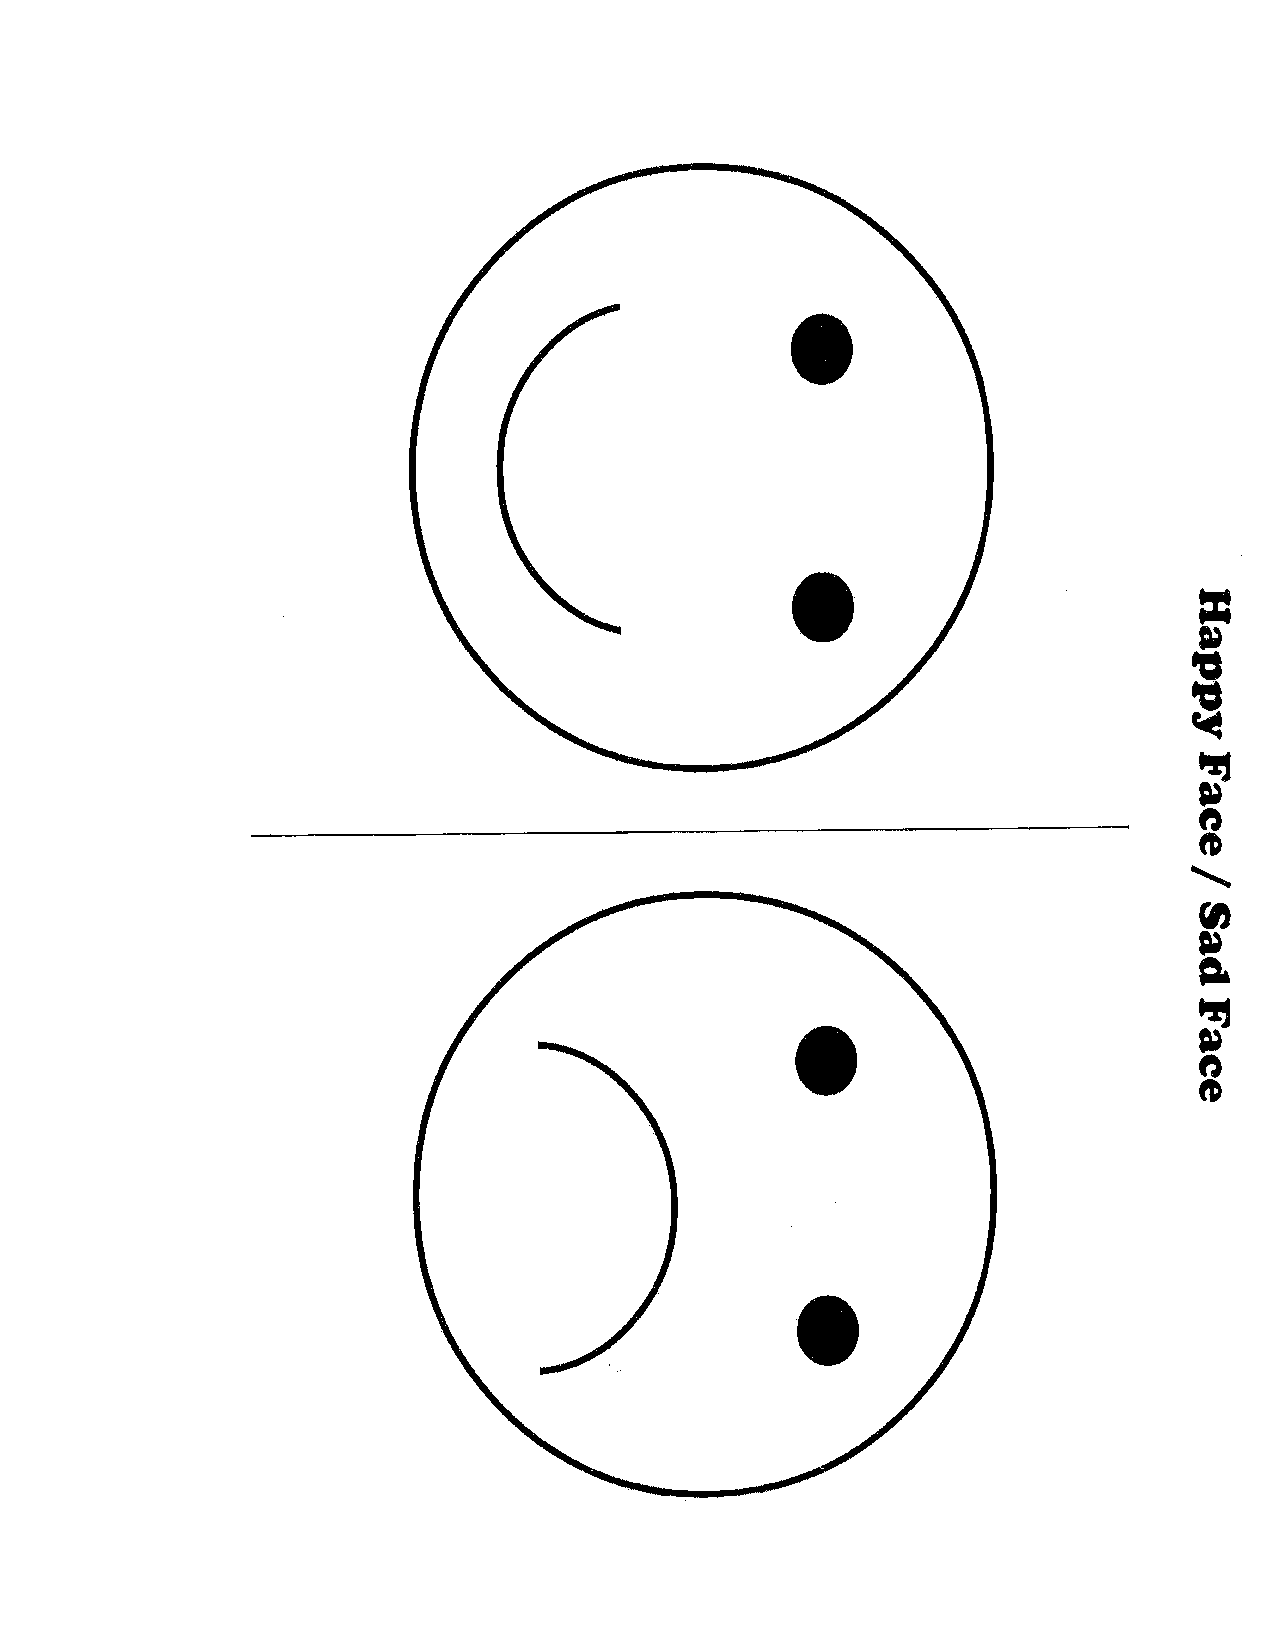
\includepdf[pages=-]{pdfs/Happy-Face-Sad-Face.pdf}

\subsection{Inserting Boxes}

We can also insert colored boxes to highlight key information

\begin{myboxb}
    \begin{definition}[Linear Programming]
       We are to find the max/ min of a linear function, subject to linear constraints:
       \begin{align}
           & \text{max/min}(c \cdot = c_1x_1 + \cdots + c_n x_n) \\
           \text{Subject to: } & Ax \geq b \\
           & x \geq 0
       \end{align}
    \end{definition}
\end{myboxb}

\begin{myboxg}
    \begin{definition}[Linear Programming]
       We are to find the max/ min of a linear function, subject to linear constraints:
       \begin{align}
           & \text{max/min}(c \cdot = c_1x_1 + \cdots + c_n x_n) \\
           \text{Subject to: } & Ax \geq b \\
           & x \geq 0
       \end{align}
    \end{definition}
\end{myboxg}

\begin{myboxr}
    \begin{definition}[Linear Programming]
       We are to find the max/ min of a linear function, subject to linear constraints:
       \begin{align}
           & \text{max/min}(c \cdot = c_1x_1 + \cdots + c_n x_n) \\
           \text{Subject to: } & Ax \geq b \\
           & x \geq 0
       \end{align}
    \end{definition}
\end{myboxr}



